\section{Framework}

Describe comms framework, plugin framework, and software
development practices.

\subsection{Communications Framework}\label{SecComms}

The \ngrm\ architecture is hierarchical and recursive
(\ref{ReqsHiLevFun}, req. 4.1).
A root instance of \ngrm\ contains all the
idle resources.  A job spawned by the root instance contains
its own \ngrm\ instance, which may in turn spawn jobs, ad infinitum.
When a job terminates, the job's instance terminates and resources
return to the parent instance.

The communications framework supports this architecture by
establishing a {\em comms session} to contain each \ngrm\ instance.
The framework enables secure, scalable communication
within a comms session, limits communication between sessions,
and allows new comms sessions to be created, resized, destroyed,
and monitored by existing ones in a parent-child relationship.

A comms session is only ``aware'' of its parent and offspring.
Any communication between siblings would have to be orchestrated by
the parent.  This abstraction should encourage higher level software
to be built that can operate at any level of recursion, thus improving
testability and facilitating research.

The communications framework consists of three main components:
the IP transport, comms toolkit, and comms message bus, layered
as shown in Figure~\ref{FigCommsLayers}.

\begin{figure}
\begin{minipage}[b]{0.45\linewidth}
\centering
\includegraphics[scale=0.30]{../fig/comms.eps}
\caption{Comms Framework Layers}
\label{FigCommsLayers}
\end{minipage}
\hspace{0.5cm}
\begin{minipage}[b]{0.45\linewidth}
\centering
\includegraphics[scale=0.30]{../fig/commstk.eps}
\caption{Comms Toolkit Layers}
\label{FigCommsTK}
\end{minipage}
\end{figure}

\subsubsection{Internet Protocol Transport}

The \ngrm\ comms framework is layered upon IP, and presumes
complete IP level unicast and multicast connectivity, so that any
collection of nodes can be wired up in a comms session without
the need to re-implement the equivalent of IP routing within
the framework.\footnote{Building a reliable 100K node IP internetwork
is a solved problem.}

The addressing, routing, and subnetting of this IP network is beyond of
scope of \ngrm, except that its design should introduce no single
points of failure (\ref{ReqsHiLevFun}, req. 1.2), should be protected
from external intrusion, and should avoid performance bottlenecks which
would unnecessarily constrain the resource manager's node selection options.

The comms framework should support communication over multiple
(fully-routed) network planes, for example using either a management
ethernet or IP-over-IB or both according to the performance/reliability
requirements of the particular application.

Dynamic unicast IP address allocation must be available to support
dynamically created virtual interfaces for Linux containers.  Similarly,
dynamic multicast address allocation must be available to support
private multicast groups within dynamically created comms sessions.
These requirements can be addressed by existing technology such as
DHCP\cite{rfc2131} and MADCAP\cite{rfc2730}.

A private DNS\cite{rfc1034} is used by the comms framework to
map a hierarchical namespace to the comms session hierarchy.
The root comms session has the root domain name, e.g. ``{\tt \ngrm.}'',
and the root server contains address records for all hosts in the domain, e.g.
``{\tt n1.\ngrm}'', ``{\tt n2.\ngrm}'',..., ``{\tt n99999.\ngrm}''.
Comms sessions spawned by the root session get their own sub-domain, e.g.
``{\tt s1.\ngrm}'', ``{\tt s2.\ngrm}'', ``{\tt s3.\ngrm}'',
and contain address records for the nodes assigned to them, e.g.
``{\tt n1.s1.\ngrm}'', ``{\tt n2.s1.\ngrm}'', ``{\tt n3.s1.\ngrm}''.
Sub-domains are created for each level of comms session recursion.
Each session runs a set of DNS servers for its domain.
When a node joins a new session, its DNS resolver is reconfigured to use
the session DNS servers and to default unqualified names to the session's
DNS domain, thus each level of session overlays a new set of names over
the root session's that provides job-centric naming uniformity.
DNS SRV records\cite{rfc2782} provide a rudimentary service location
brokerage within the session.
Well understood techniques for DNS fault tolerance,
caching, and dynamic reconfiguration are leveraged to scale performance
in large sessions such as the root session.


\subsubsection{Comms Toolkit}

The framework provides a toolkit for sending and receiving
protocol messages privately and securely within a session,
with the goals of providing a robust foundation for \ngrm\ components
and promoting rapid development, code reuse, and interoperability.
The toolkit includes a messaging library,
protocol encoding/decoding libraries, and a security framework.
Toolkit pieces can be mixed and matched according to application requirements.

0MQ\cite{ZMQGuide} is a messaging library that
provides the ability to manipulate opaque, multipart messages, and
carry them across various transports, including TCP and PGM\cite{rfc3208}
(reliable multicast), using a socket-like API.  0MQ sockets can
exchange messages using various {\em patterns},
including REQ-REP (RPC), PUB-SUB, and PUSH-PULL (message stream).
0MQ can be used to build applications or custom message brokers.
Complex message routing topologies such as tree-based overlay networks
(Figure~\ref{FigZmqTBON}) can be built from simple components.
0MQ has a large number of language bindings.

\begin{figure}
\centering
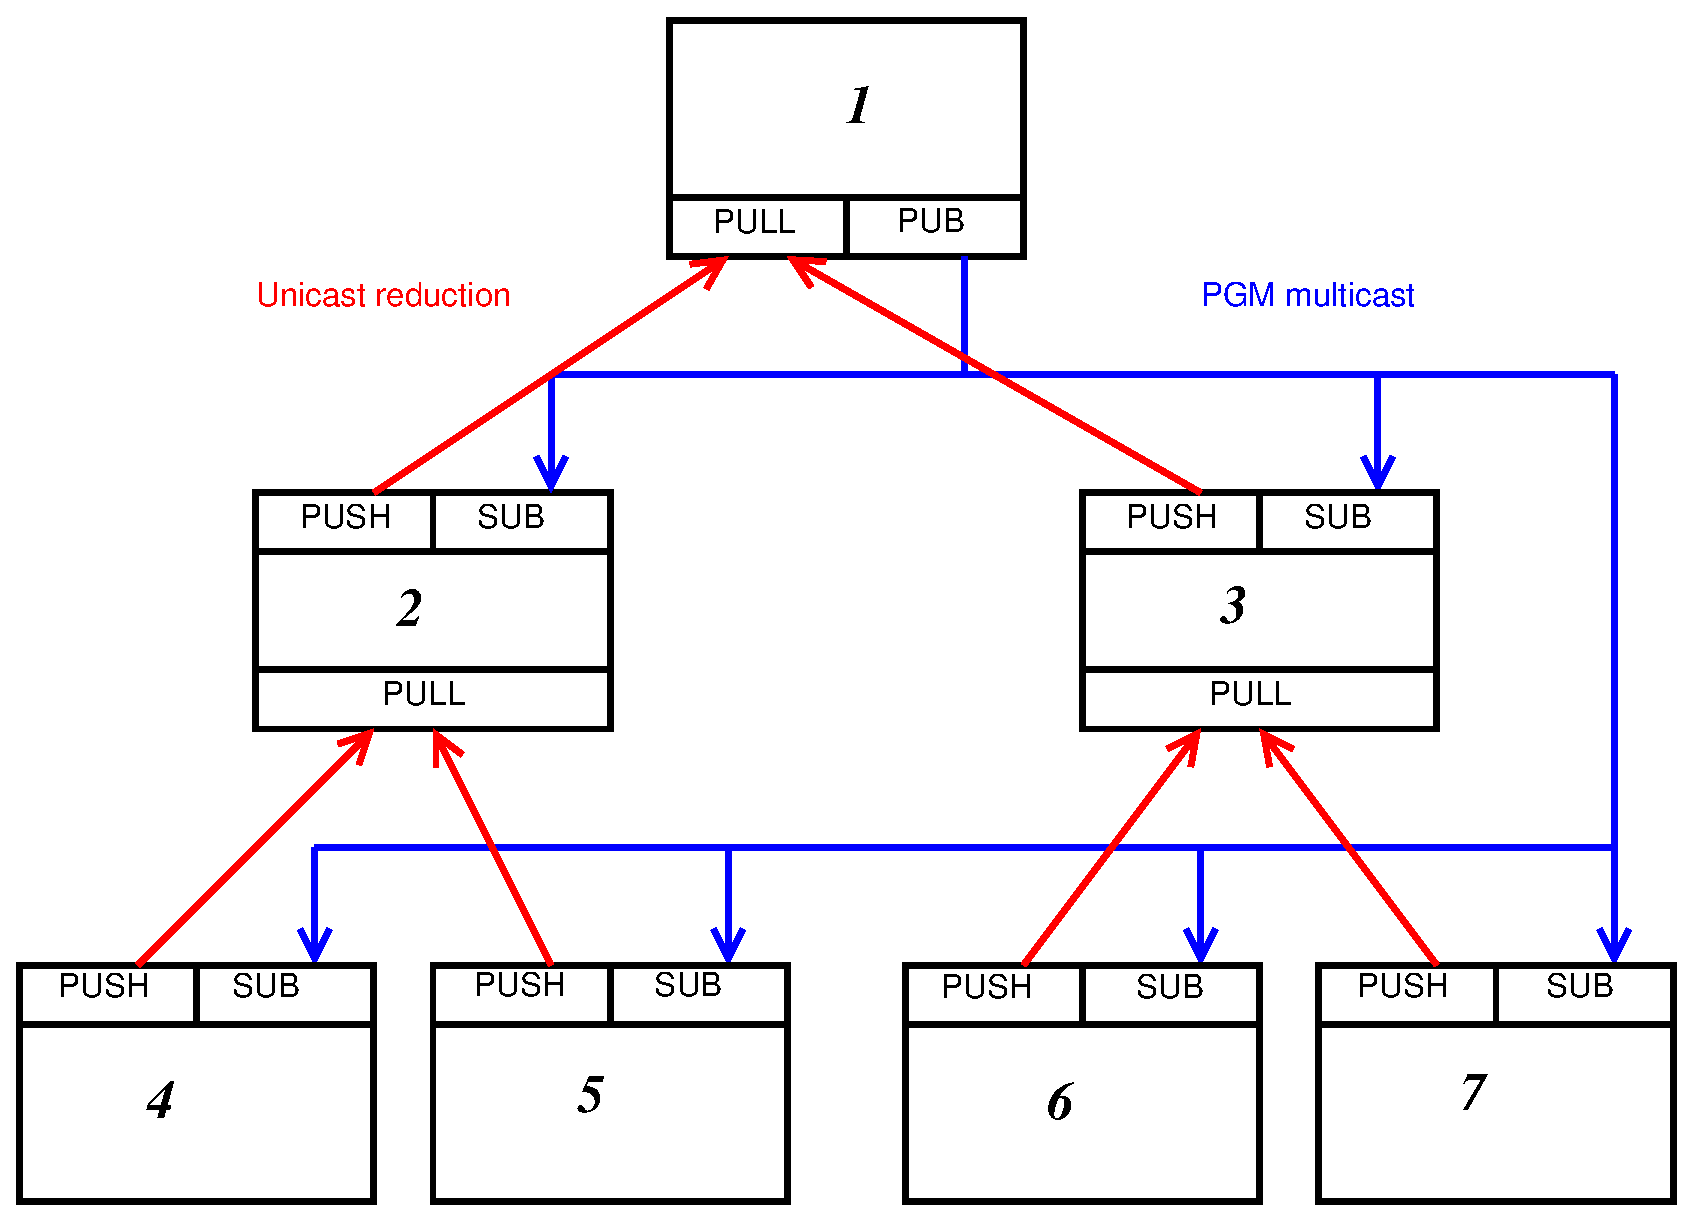
\includegraphics[scale=0.35]{../fig/zmqtbon.eps}
\caption{Tree Based Overlay Network Over 0MQ}
\label{FigZmqTBON}
\end{figure}

Two widely used methods of encoding data in messages are
JSON\cite{rfc4627} 
and Protocol Buffers\cite{Protobuf}.
JSON is a self-describing format
that supports protocol evolution without recompiling endpoints.  It has
many language bindings but it is also space-inefficient and slow.
Protocol Buffers is a compiled format that supports
only limited protocol evolution without recompilation.  It has relatively
fewer language bindings than JSON but is space-efficient and fast.
Depending on the application either may be appropriate.

Messages can be secured with a session-wide security context.
Each comms session is allocated a {\em session key} by its parent\footnote{
The root comms session obtains its session key out of band.}
which is used for establishing a shared security context
for messages exchanged within the comms session.
The shared security context allows communicating entities to have integrity
and privacy (from children, siblings, and their children)
without the overhead
of a key exchange for each pair of communicating endpoints.
This is especially useful for non point-to-point comms patterns such as PUB-SUB.
The parent retains state about its offspring including their session keys.
Children lose access to their parent's key;  thus as comms sessions recurse,
parents get privacy from children but not the reverse.
An application acting as a gateway between parent and child would use
the child's session key as it is known by both parent and child.

Alternatively, messages can be enclosed as payload in a MUNGE\cite{MUNGE}
credential when authentication of the sending user is required,
at the cost of an exchange with the MUNGE daemon on both ends.
This also provides intergrity and privacy for the message that
is robust to threats from within the comms session.
In order for this to work, \ngrm's comms framework must operate within a
single MUNGE security realm,\footnote{MUNGE must acquire the ability
to update its shared secret without introducing downtime. FIXME: ref bug\#}
which implies a single single administrative domain with consistent
user and group identities.

\subsubsection{Comms Message Bus}\label{SecCommsCMB}

Within a comms session, a distributed comms message bus\footnote{
Although we refer to it as a message bus because its function
is analagous to that of system-dbus on Linux, the CMB topology is to
be determined.  For large sessions, a tree is more likely than a bus.}
service (CMB), is established for lightweight monitoring and session control.
A distinguished {\em control node} acts as a gateway between the
session's CMB and the parent session's CMB.  Interfaces exposed to the
parent are passive; that is, the parent initiates connections and
makes requests or subscribes to data, and the child control node
responds or publishes data.  The CMB implements the functions shown
in Table~\ref{TabCMBFun}.

\begin{table}
  \centering
  \begin{tabular}{| l | p{0.6\textwidth} |}\hline
  \textbf{Function} & \textbf{Description} \\
  \hline
  $cmb\_trigger\_wait $ &
	Sleep until session trigger or maximum wait time elapses. \\
  $cmb\_trigger\_get/set$ &
	Get/set session trigger period.
	Optionally set random delay bound to tune jitter.\\
  \hline
  $cmb\_liveness\_get$ &
	Get node liveness. \\
  $cmb\_liveness\_sub/unsub$ &
	Subscribe/unsubscribe to node liveness updates. \\
  \hline
  $cmb\_nodeset\_get$ &
	Get nodeset. \\
  $cmb\_nodeset\_add/del$ &
	Add/delete node to/from nodeset. \\
  $cmb\_nodeset\_sub/unsub$ &
	Subscribe/unsubscribe to nodeset updates. \\
  \hline
  $cmb\_session\_create/destroy$ &
	Create/destroy a comms session. \\
  \hline
  plugin interfaces &
	TBD. \\
  \hline
  \end{tabular}
  \caption{Comms Message Bus Functions}
  \label{TabCMBFun}
\end{table}
%

The CMB provides a session-wide periodic, multicast {\em trigger signal}
which enables events, including CMB's internal functions, to be cooperatively
scheduled across the session to minimize disruption to bulk-synchronous
workloads.  The trigger period is tunable for individual sessions.
Higher level software running anywhere in the session has access to
this trigger signal.

The CMB implements a lightweight monitoring and membership service.
The {\em liveness} state of member nodes is assessed by forcing
them to communicate with the CMB at minimum intervals,
synchronized by the trigger signal.
If the CMB has not heard from a node for some number
of trigger signal periods, it is marked {\em down}, and eventually may
be evicted from the session.  Higher level software running anywhere in
the session can obtain the current {\em nodeset} and liveness state
by request, and can subscribe to notification when the nodeset changes
or when the liveness state of any nodes change.
The parent continues to track liveness of nodes allocated to a child by
subscribing to liveness updates via the child's control node.  A trivial
utility that asks the CMB for a list of down nodes in the current session
can be written that works equally well at any level of recursion,
even at the level of the root session.

The CMB maintains the current nodeset and mirrors it in the session DNS
domain.  The CMB can add or delete nodes from the nodeset on request
from the local session or from the parent.  The CMB does not offer a
mechanism a sessions to {\em request} nodes from the parent; this
is left to a higher software layer.  Nodes retain a stack of comms
session contexts, so that a node added to a child session pushes the current
session context, and, when relinquished by the child, can pop the parent
context and reconnect.
While nodes are allocated to the child, they remain in the parent nodeset
and DNS domain but the CMB tags them as allocated.  Unless they are the
distinguished control node, allocated nodes do not communicate directly with
the parent CMB or listen to the parent's trigger signal.

When the CMB first starts up on a node, it obtains information about its
comms session out of band.
A real node would join the root session, while a dynamically created
container instance would join the comms session of the host node.
When a node crashes and reboots, it tries to join the root session and if
it had been allocated to a child session, is re-added from child to
child until it reaches its current owner.  A node re-added in this manner
can be accepted or evicted according to the session's policy.

\begin{figure}
\centering
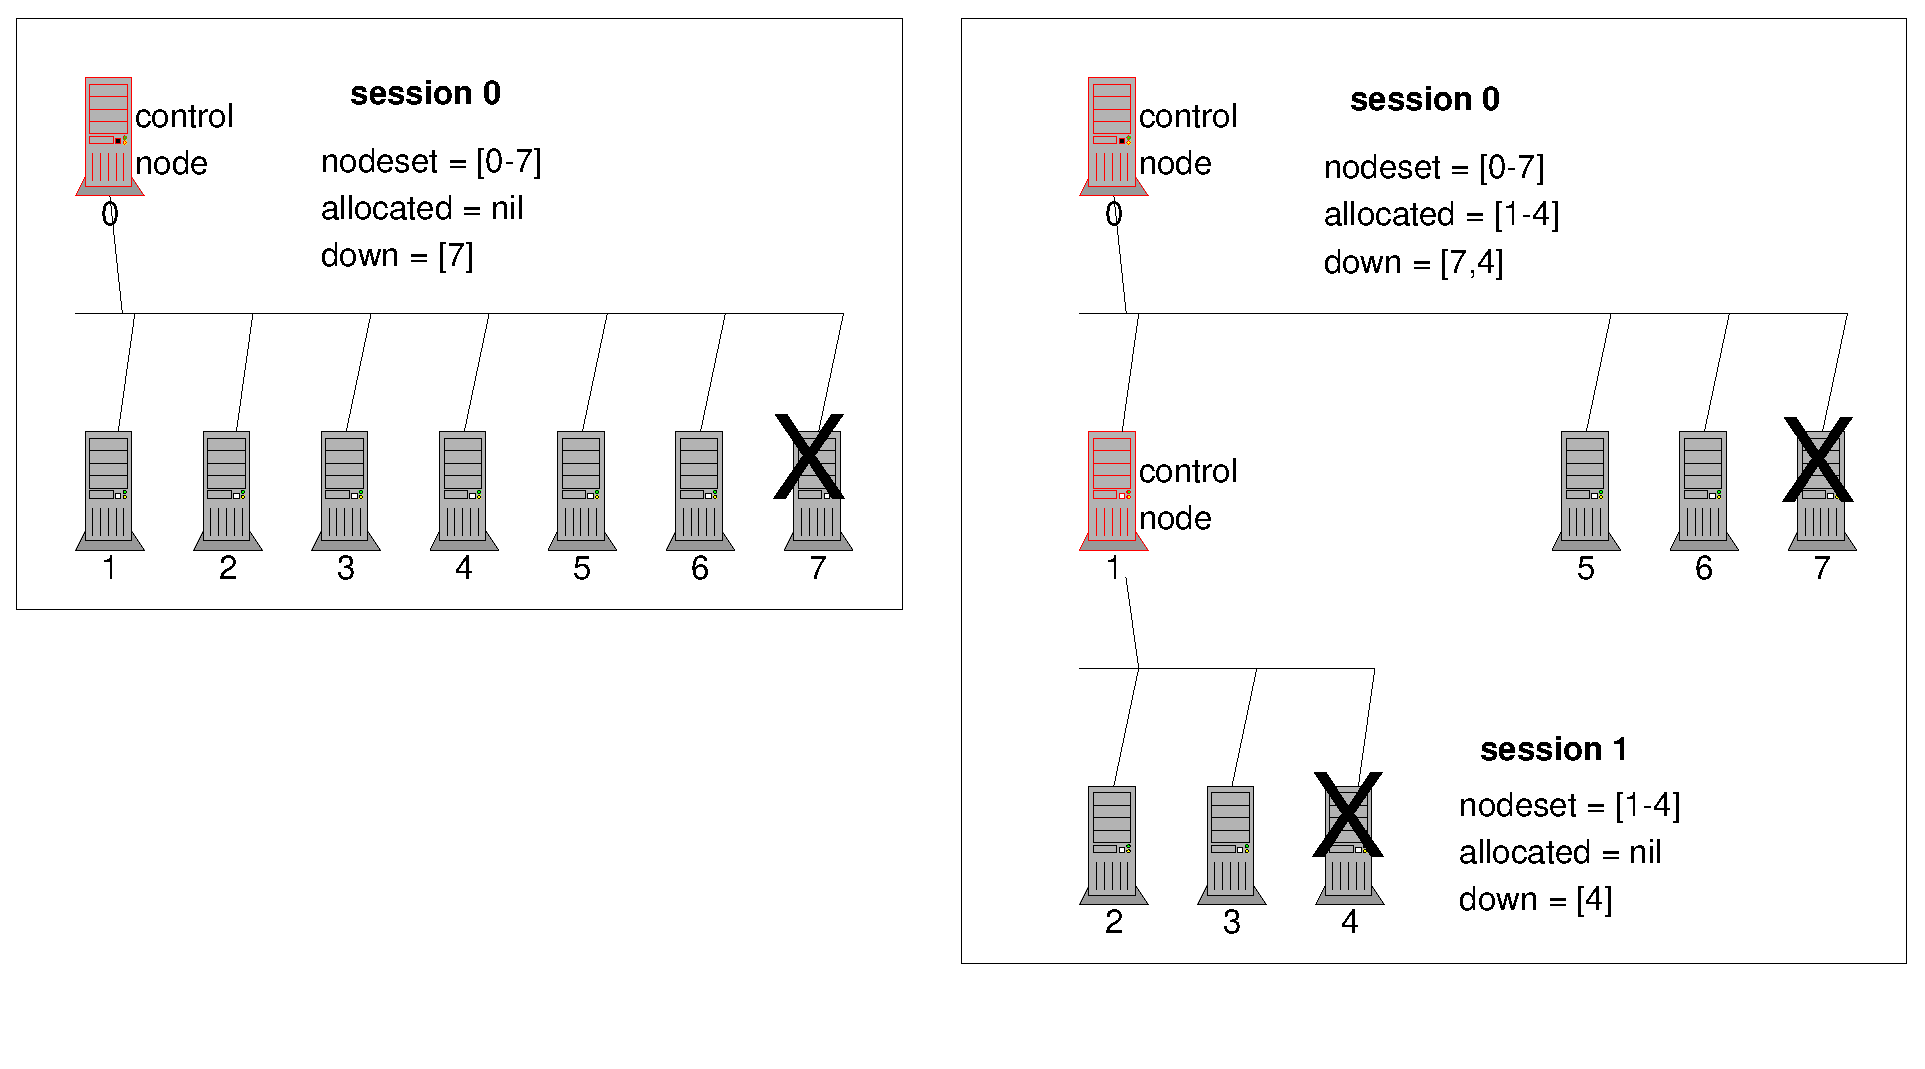
\includegraphics[scale=0.50]{../fig/cmb.eps}
\caption{Comms Message Bus Spawning a New Comms Session}
\label{FigCMBSpawn}
\end{figure}

The CMB is responsible for the creation and destruction of
comms sessions as shown in Figure~\ref{FigCMBSpawn}.
A new session is created with a CMB request that
includes the new nodeset and identifies the control node.  The CMB
generates the session context and topology and passes it to the nodes
in the nodeset, which wire up a new CMB instance for the session.
Creation of a session also involves the update of DNS information
in the parent and the establishment of DNS servers and resolver updates
in the child. 
A session is destroyed with a CMB request to the session,
which can originate from the parent or the within the session itself.
In the event that the control node for the session to be destroyed has become
unresponsive, it is possible for the parent to send the session a
special multicast trigger signal indicating that the session nodes
should exit the current session immediately.

Finally, although the CMB is not intended to be {\em the} shared messaging
framework for the session, it can be extended using plugins.
For example it may be desirable to implement logging, remote execution,
framework bootstrapping, or container instance creation using the
CMB framework.  The design of a plugin architecture for CMB is TBD.
